\subsection{Flickr}
Foto�s kunnen naar Flickr worden ge�pload via het overzicht File operations in de 
persoonlijke Workbench. Ga hiertoe als volgt te werk:

1. Open het overzicht
\begin{figure}[p]
\centering
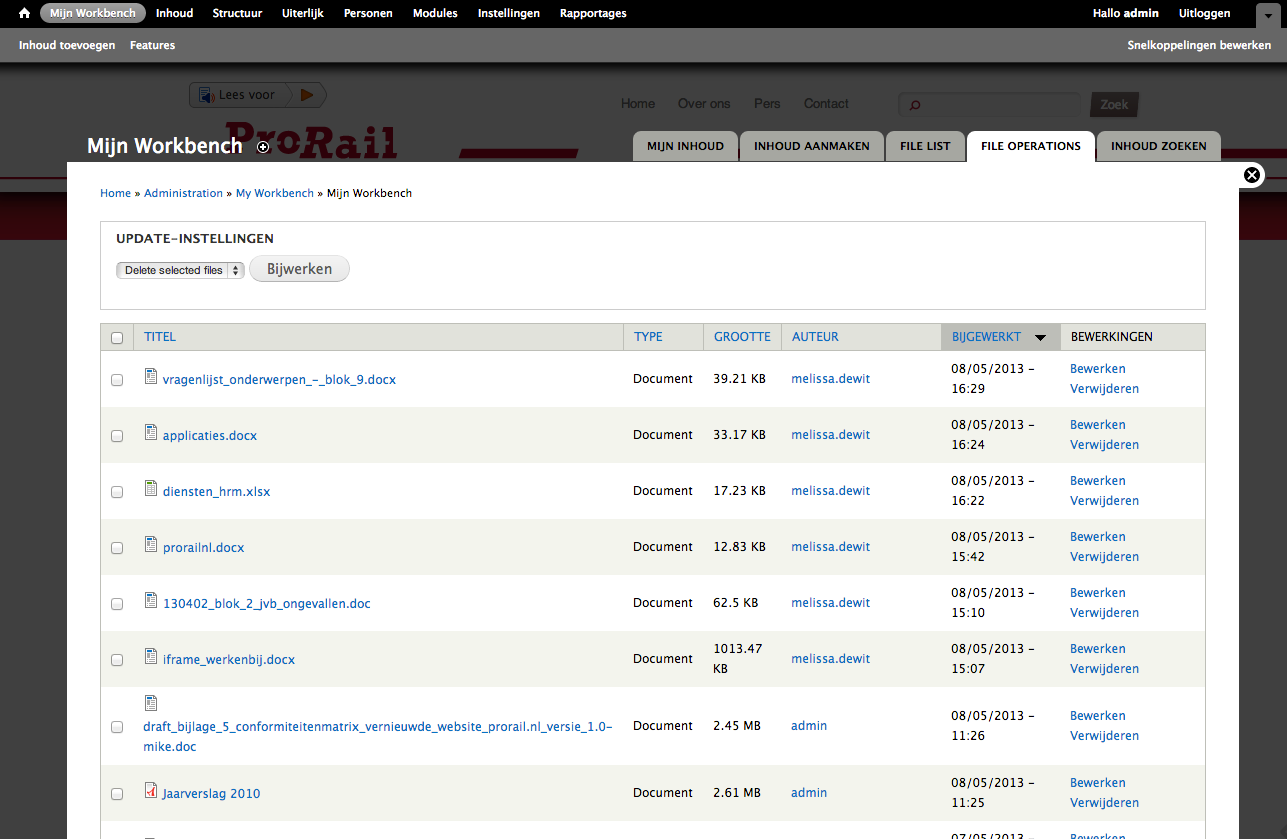
\includegraphics[width=\textwidth]{img/flickr/flickr_file_operations.png}
\end{figure}

2. Vink de bestanden aan die ge�pload moeten worden.
\begin{figure}[p]
\centering
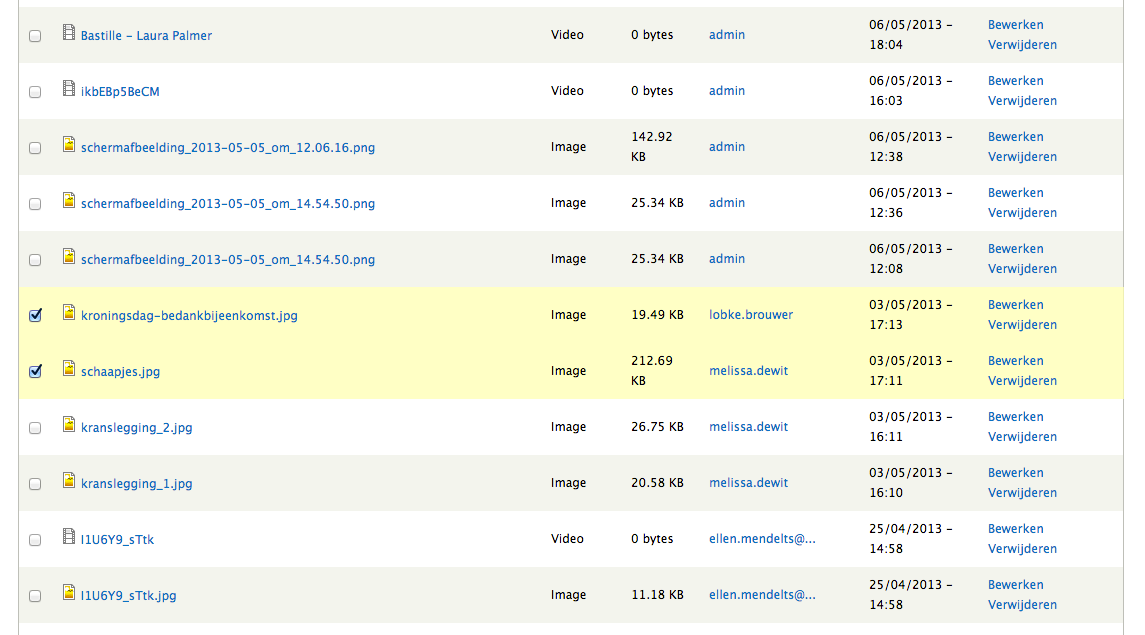
\includegraphics[width=\textwidth]{img/flickr/flickr_selecteren.png}
\end{figure}

3. Selecteer bovenaan in de dropdown �Upload naar Flickr� en druk op Bijwerken.
\begin{figure}[p]
\centering
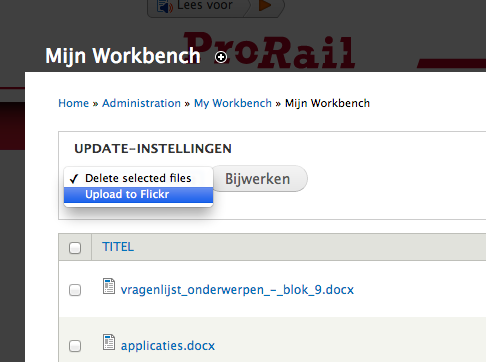
\includegraphics[width=\textwidth]{img/flickr/flickr_upload.png}
\end{figure}

4. Het systeem zal redirecten naar Flickr en vragen om een login. Log in voor de Flickr 
account waar naartoe ge�pload moet worden. Geef toestemming.
\begin{figure}[p]
\centering
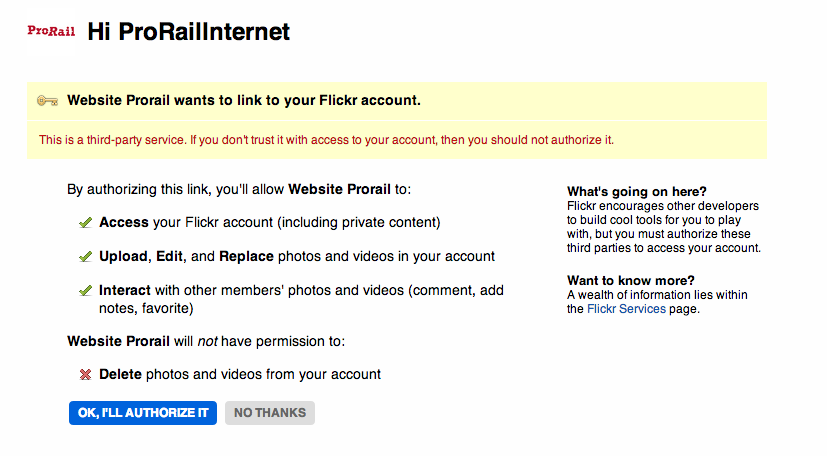
\includegraphics[width=\textwidth]{img/flickr/flickr_login.png}
\end{figure}

De afbeeldingen worden ge�pload en u komt weer terug in het File operations overzicht.